% SSU Data Dash 2026 report. Compile on Overleaf (pdfLaTeX) with the three .png files in the
% same folder. The only thing left to fill in is the video link (in red).

\documentclass[11pt,a4paper]{article}

\usepackage[margin=1.8cm,bottom=2.4cm,footskip=1.1cm]{geometry}
\usepackage{amsmath}
\usepackage{lmodern}
\usepackage{mathptmx}
\usepackage[T1]{fontenc}
\usepackage{microtype}
\usepackage[dvipsnames]{xcolor}
\usepackage{graphicx}
\usepackage{booktabs}
\usepackage{tabularx}
\usepackage{caption}
\usepackage{float}
\usepackage{titlesec}
\usepackage{fancyhdr}
\usepackage{lastpage}
\usepackage{listings}
\usepackage{needspace}
\usepackage[colorlinks=true,urlcolor=NavyBlue,linkcolor=black]{hyperref}

\linespread{1.1}
\setlength{\parindent}{0pt}
\setlength{\parskip}{0.5em}

\definecolor{rule}{HTML}{C8C8C8}
\definecolor{footer}{HTML}{4A5A78}
\titleformat{\section}{\large\bfseries}{\thesection.}{0.4em}{}[{\vspace{-0.45em}\color{rule}\titlerule[0.6pt]}]
\titleformat{name=\section,numberless}{\large\bfseries}{}{0em}{}
\titlespacing*{\section}{0pt}{0.9em}{0.5em}

\pagestyle{fancy}
\fancyhf{}
\renewcommand{\headrulewidth}{0pt}
\renewcommand{\footrulewidth}{0.4pt}
\renewcommand{\footrule}{{\color{rule}\hrule width\headwidth height\footrulewidth}\vskip 4pt}
\fancyfoot[L]{\small\color{footer}SSU Data Dash 2026 Submission Report}
\fancyfoot[R]{\small\color{footer}Page \thepage\ of \pageref*{LastPage}}

\captionsetup{font=small,labelfont=bf,labelsep=colon,skip=4pt}
\lstset{basicstyle=\ttfamily\small,backgroundcolor=\color{gray!8},frame=single,
        rulecolor=\color{gray!20},breaklines=true,columns=fullflexible,
        xleftmargin=4pt,xrightmargin=4pt,aboveskip=4pt,belowskip=0pt}

\begin{document}

\begin{center}
  {\LARGE\bfseries SSU Data Dash 2026}\\[6pt]
  {\itshape Indy Ou, John Sakalli, Nyle Hassan Kazmi}
\end{center}
\vspace{-4pt}
{\color{black}\hrule height 0.8pt}
\vspace{6pt}
{\small
\begin{tabularx}{\textwidth}{@{}p{0.43\textwidth}X@{}}
\textbf{Video (YouTube, unlisted is fine):} & \url{https://youtu.be/MpkyyfFby_I}\\[2pt]
\textbf{Code \& submission files (GitHub):} & \url{https://github.com/Indy801/SSU-Data-Dash/}\\
\end{tabularx}}

% ======================================================================================
\section*{Summary}

We predict Toronto home sale prices on two tracks: off-market, with no list price (for owners
and lenders valuing a home before listing), and list-aware, with the list price (for buyers
deciding what to offer). Our final model blends two gradient-boosted tree models trained on the
log of the sale price. Under walk-forward validation from December 2025 to May 2026 (10,069
homes per track, each month predicted only from earlier sales), it reaches an MdAPE of 7.59\%
off-market, against 14.87\% for the starter gradient-boosted model, 20.84\% for the starter
nearest-sales baseline and the 17.7\% points bar. List-aware MdAPE is 4.06\%, against 4.61\% for
the starter model and 7.26\% for the list price alone. Error is lowest for mid-priced homes and
highest for the most expensive tenth, where one off-market prediction in four misses by more
than 20\%.

% ======================================================================================
\section{Data and features}

Every model starts from the starter features: floor area in square feet (the number, or the
midpoint when the listing gives a range), bedrooms, washrooms, total parking, the home's
latitude and longitude, months since January 2021 to capture market trends, and one indicator
for each of the six property types. Days on market and the external AVM estimate were not
used, because both exist only after a sale, and we used no outside data.

% ======================================================================================
\section{Models}

We compared eleven alternatives on both tracks under the same validation
(Figure~\ref{fig:models}): the starter baseline, random forests on price and on log price, a
multilayer perceptron (MLP) on log price, the starter's gradient-boosted trees, and XGBoost and
LightGBM, each plain, with listing-remarks text, and with imputation of missing values.

Our final model blends two gradient-boosted tree libraries, \textbf{LightGBM and CatBoost},
averaging their predictions of $\log(\mathit{sale\ price})$. Recent sales are weighted more
heavily (a sale a year older counts half as much), because the data spans the 2021--22 boom and
the correction after it, and obvious data errors are removed from the training sales before
each fit. For the \textbf{list-aware track}, the model predicts
$\log(\mathit{sold\ price} / \mathit{list\ price})$, how far above or below asking a home sells,
and applies that to the list price.

% ======================================================================================
\section{Validation}

We used the starter code's walk-forward validation (\texttt{run.py validate}). For each month
from December 2025 to May 2026, a model is trained only on sales before that month and predicts
the homes sold in it, with the sold price, sale date, days on market and AVM fields hidden (and,
off-market, the list price). Every model is scored on the same 10,069 homes per track by MdAPE,
with 95\% bootstrap intervals from 1,000 resamples. Hyperparameters for XGBoost, LightGBM and
our final model were tuned on these same months, so their scores may be slightly optimistic.
Each validation month is also only one month past its training data, while the hidden test runs
one to four months past it, so we expect the hidden-test error to be somewhat higher than the
figures below.

% ======================================================================================
\needspace{16\baselineskip}
\section{Results}

\begin{table}[H]
  \centering
  \small
  \begin{tabularx}{\textwidth}{@{}Xrrcr@{}}
    \toprule
    \textbf{Model Track} & \textbf{MdAPE (\%)} & \textbf{MAPE (\%)} & \textbf{95\% CI (MdAPE)} & \textbf{Median signed error (\%)}\\
    \midrule
    Off-Market (Starter: Nearest Sales)      & 20.84 & 27.43 & [20.40, 21.36] & +8.07\\
    Off-Market (Starter Gradient Boosting)   & 14.87 & 19.23 & [14.50, 15.23] & +1.02\\
    Off-Market (Final Model)                 & \textbf{7.59} & \textbf{9.92} & [7.43, 7.77] & $-$0.01\\
    \midrule
    List-Aware (Starter: List Price)         & 7.26 & 8.09 & [7.12, 7.41] & +5.68\\
    List-Aware (Starter Gradient Boosting)   & 4.61 & 5.82 & [4.50, 4.71] & +0.68\\
    List-Aware (Final Model)                 & \textbf{4.06} & \textbf{5.14} & [3.98, 4.15] & +0.20\\
    \bottomrule
  \end{tabularx}
  \caption{Walk-forward validation, December 2025 to May 2026, 10,069 homes per track. MdAPE:
  median absolute percentage error. MAPE: mean absolute percentage error. Brackets: bootstrap
  95\% confidence interval. Signed error above 0 means the model predicts too high.}
  \label{tab:results}
\end{table}

The final model is best on both tracks (Table~\ref{tab:results}, Figure~\ref{fig:models}).
Off-market, it cuts MdAPE by 64\% against the nearest-sales baseline and by about half against
the starter model; the next best alternative, LightGBM with imputation, reaches 8.63\%.
List-aware, it reaches 4.06\%, against 4.33\% for the next best. No interval overlaps its
neighbour's, so these gaps are not resampling noise. The final model's median signed error is
near zero on both tracks, while the baselines predict too high by 8.1\% and 5.7\%: earlier
nearby sales overstate later prices, and homes sold at a median of about 5\% below asking.
Adding raw listing-remarks text made both XGBoost and LightGBM worse.

\begin{figure}[H]
  \centering
  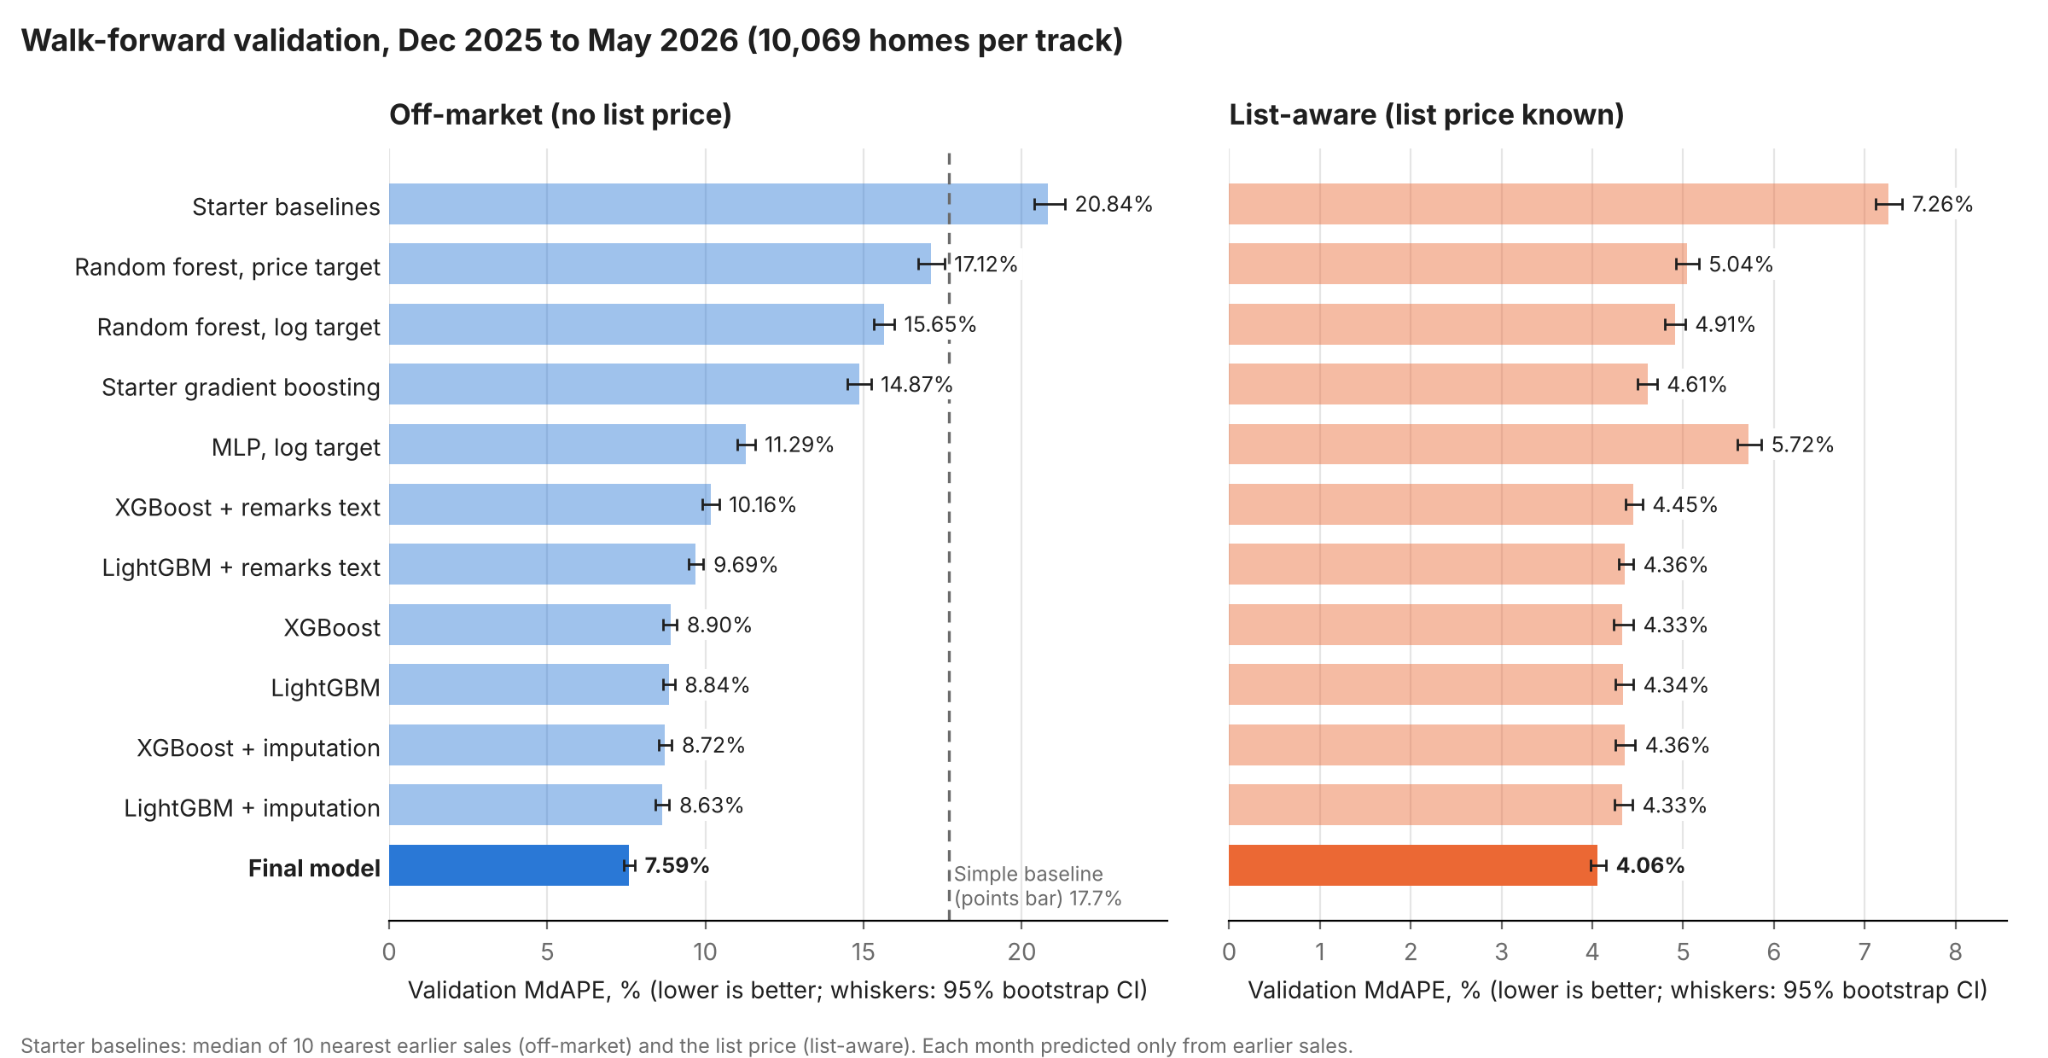
\includegraphics[width=0.97\textwidth]{model_comparison.png}
  \caption{Validation MdAPE of every model, off-market (left) and list-aware (right). Whiskers:
  95\% bootstrap intervals; dashed line: the 17.7\% points bar.}
  \label{fig:models}
\end{figure}

% ======================================================================================
\section{Where the model fails}

Figure~\ref{fig:price} breaks the error down by sold-price decile. Our model has lower error than
the starter model in every decile on both tracks, but the pattern is the same: errors are
largest at the ends of the price range. Off-market error is lowest for mid-priced homes, about
6\% in deciles 2--4, and climbs to about 13\% in the top decile (median \$2.34M), where one
prediction in four misses by more than 20\%. These homes are rarer, so each has fewer comparable
sales, and their price rests on finishes and design details the data barely records. The
cheapest decile (about 7.5\%) is also harder than the middle, since a small dollar miss on a low
price is a large percentage. List-aware error stays near 3.5\% for cheaper homes and reaches
about 5.7\% at the top, where negotiation moves prices further from asking.

\begin{figure}[H]
  \centering
  \begin{minipage}{0.49\textwidth}\centering
    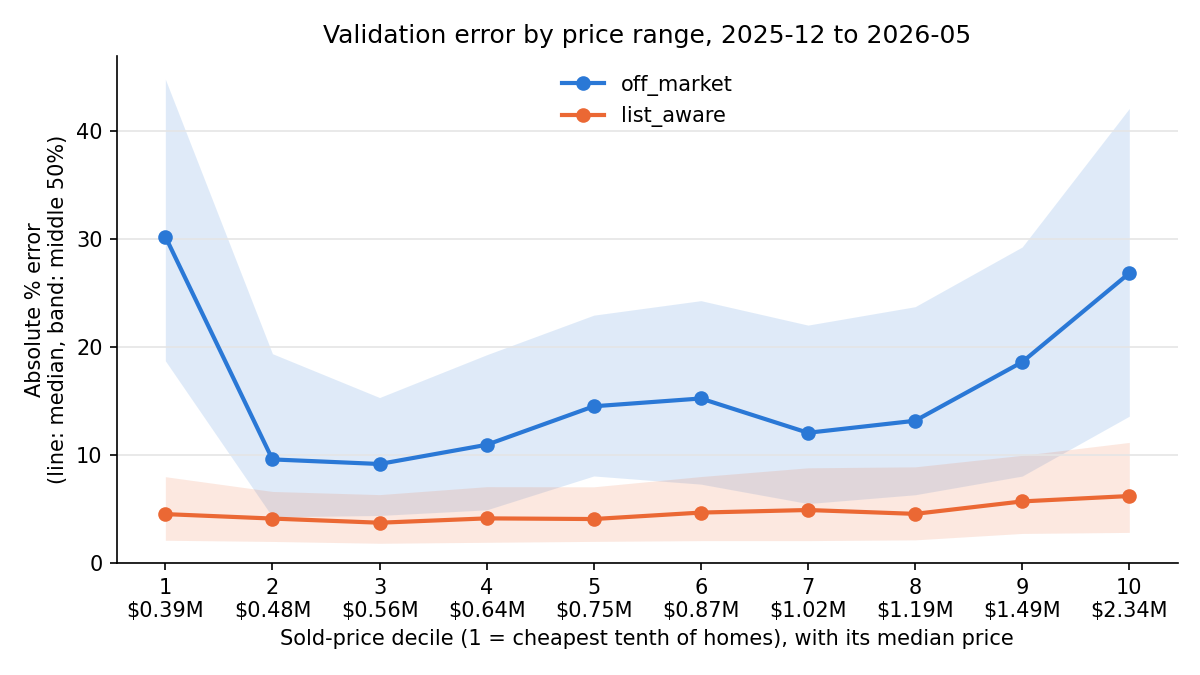
\includegraphics[width=\textwidth]{error_by_price_starter.png}\\[-2pt]
    {\small (a) Starter gradient-boosted model}
  \end{minipage}\hfill
  \begin{minipage}{0.49\textwidth}\centering
    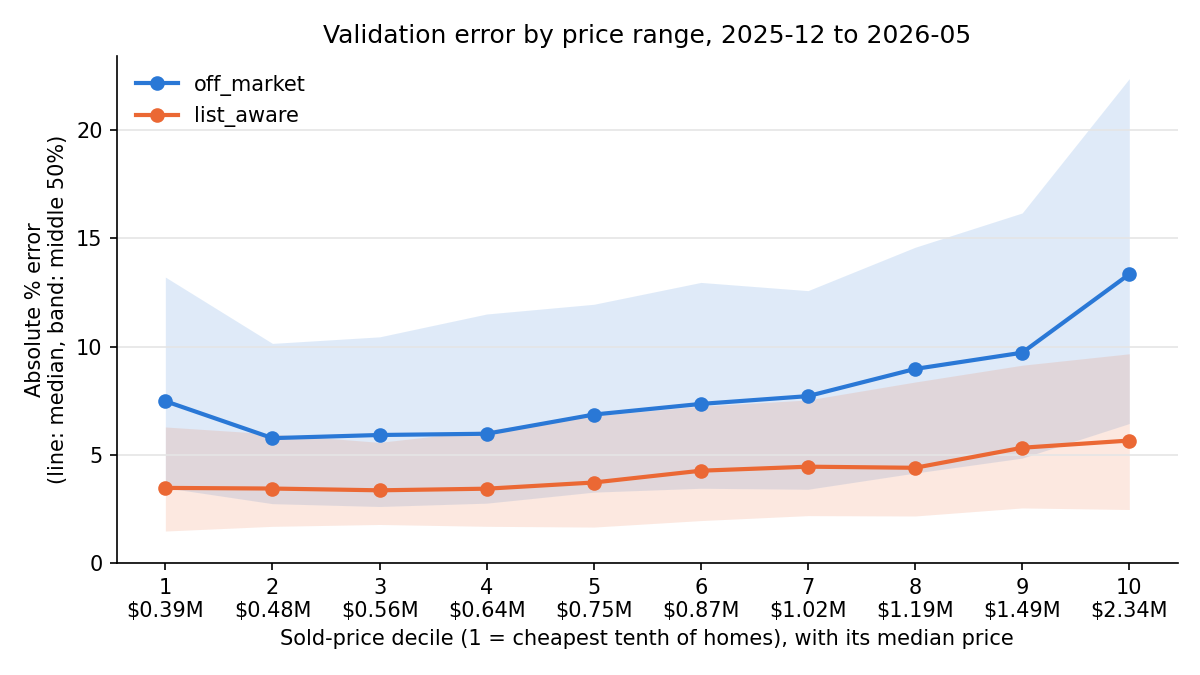
\includegraphics[width=\textwidth]{error_by_price_final.png}\\[-2pt]
    {\small (b) Our final model}
  \end{minipage}
  \caption{Absolute percentage error by sold-price decile (1 = cheapest tenth of homes). Line:
  median; band: middle 50\%. Note the different y-axis scales: the starter model's goes twice
  as high.}
  \label{fig:price}
\end{figure}

% ======================================================================================
\section{Limitations}

The model cannot see market moves after May 2026: trees hold the price level at the last months
they saw, so a decline or rebound between June and September shifts every prediction by
roughly that move. It should not be relied on alone for the most expensive homes or for
communities with few sales, where comparable sales or an appraiser are needed. Because
hyperparameters were tuned on the validation months, our validation error may slightly
understate the hidden-test error. The data is synthetic, so these errors show the method rather
than accuracy on real Toronto sales, and the model gives one number per home with no range.
Next, we would add comparable-sales features, quantile models that give each home a price range,
and tuning on months before December 2025 so the validation months stay untouched.

% ======================================================================================
\section*{Outside data}

Outside data is not used during the building of models.

\section*{Reproducing our results}

\begin{lstlisting}
pip install -r requirements.txt
python run.py validate && python run.py report
python run.py predict && python run.py check
\end{lstlisting}

\end{document}
